\section{Monte Carlo Simulations}
\label{htcc-sim-sec}

Comprehensive Monte Carlo (MC) simulations to check the major parameters of the HTCC were done before the
design of the detector was completed. Electrons of 2~GeV energy were used. The core concept of the goal to
reach was to build a detector that had to be installed in front of the forward tracking system as one unit without
any support structure in the acceptance. A light collection pattern has been simulated for the exact HTCC
geometry of all components, including their properties and detailed  specifications of materials to answer the
following basic questions with regard to the detector:

\begin{itemize}
\item Is the chosen light collection geometry adequate to provide the highest possible electron detection efficiency
  and efficient rejection of background events?
\item Which components (options) would provide acceptable performance of the detector (mirrors, PMTs)?
\item What shape (convex or flat) of the PMT window has the most efficient light collection?
\item What window material has to be used to provide the highest possible signal strength?
\item What are the actual image dimensions in the focal planes?
\item What would be the basic dimensions of a Winston cone light concentrator, if we had to use them?
\end{itemize}

Figure~\ref{fig:PROPERTIES} shows the MC simulation results for the properties of the major components of the
detector: transparency of the CO$_2$ radiator gas, reflectivity of the mirrors deposited with metal aluminum
covered by MgF$_2$ protection coating, and the transparency of the PMT entry window material as a function of
wavelength. The radiator gas and mirror show good optical properties (transmittance and relativity) in the UV
range.

As far as the entry window material is concerned, the quartz window provides a larger signal as compared
to a window made of UV-transmitting glass. However, PMTs with quartz entry windows are significantly more
expensive and are also fragile. We have run comparative tests of 5-in ET 9823 PMTs with both quartz and
UV-transmitting glass windows to justify our choice. Figure~\ref{fig:Quartz_UV_glass} shows the results obtained
for the PMT glass transparency. The measurements showed that average signal from a PMT with a quartz window
is equivalent to 55.6 photoelectrons, whereas for the PMT with UV-transmitting glass, the average signal is only
38.2 photoelectrons (i.e. $\sim$45\% more light for the quartz PMTs).

\begin{figure}[!ht]
    \centering
    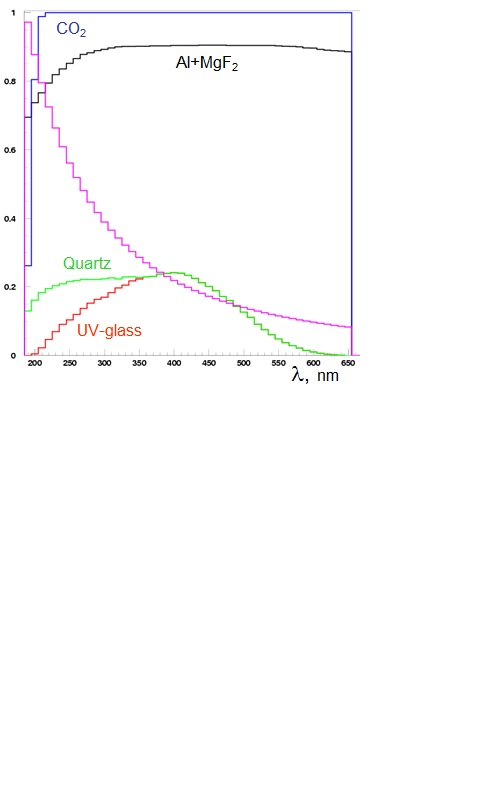
\includegraphics[width=1.0\linewidth,trim={0.0cm 10.7cm 3.7cm 0.1cm},clip]{images/PROPERTIES.jpg}
    \caption{Optical properties of the HTCC major components in terms of transparency vs. wavelength from MC
      studies. The exponential histogram (magenta) describes the Cherenkov light spectrum. The blue histogram
      shows results for the transparency of CO$_2$ gas and the black histogram shows the reflectivity of the mirror.
      The results for the response of the PMTs with a quartz face plate (green) and with a UV-transmitting glass
      window (red) are shown as well.} 
    \label{fig:PROPERTIES}
\end{figure}

\begin{figure}[!ht]
    \centering
    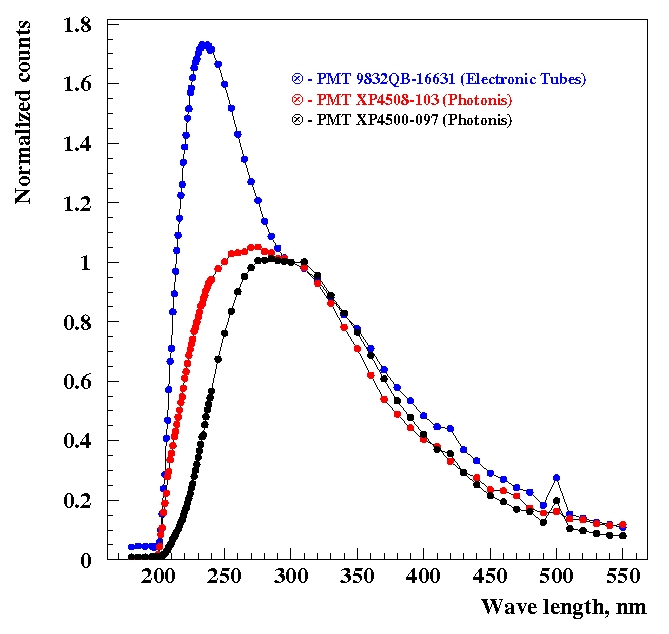
\includegraphics[width=1.0\linewidth,trim={1.7cm 0.5cm 0.05cm 0.1cm},clip]{images/Quartz_UV_glass.jpg}
    \caption{Comparative measurement test results on the transparency of PMT windows made of quartz (blue),
      UV-transmitting glass (red), and regular glass (black).}
    \label{fig:Quartz_UV_glass}
\end{figure}

In the HTCC, Cherenkov light is generated along the entire length of a scattered electron's trajectory in the volume
of the detector. The light collection geometry provided by the fully ellipsoidal mirror with point-to-point focusing is
valid only in the case when one focal point is in the target position and when the second focal point is at the face of
the PMT. Consequently, one must expect considerable changes in the size of the image in the focal plane due to the
continuous evolution of the light emission point along the electron trajectory. Moreover, there is no light emitted by
a scattered electron moving from the target until it crosses the entry window of the HTCC. PMTs of large size are
available with a face plate (entry window) of various shapes. This is one more parameter to check.

Figure~\ref{fig:Flat_Convex} shows simulation results on the collection of light impinging on the entry window for two
different PMTs, comparing those with convex windows and those with flat windows. Clearly the flat entry window is
preferable. Most of the light has larger angles of incidence for the PMTs with a convex window. Besides,
for them a larger portion of the light would undergo two reflections (off the mirror and Winston cone), whereas for
the PMTs with a flat face plate, most of the light hits the window under small angles of incidence. From
Fig.~\ref{fig:Flat_Convex} we also estimated that about 80\% of the Cherenkov light will directly impinge on the
PMT photocathode and the remaining 20\% will first be reflected by the Winston cone. The 5-in quartz ET-9823QKB
PMT used in the HTCC has a photocathode that is actually 110~mm in diameter ($\sim$4.3~in). 

\begin{figure}[!ht]
    \centering
    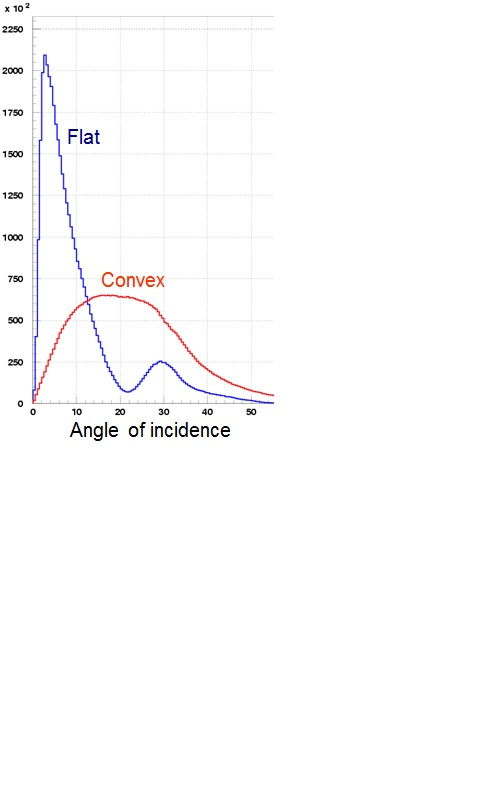
\includegraphics[width=1.0\linewidth,trim={0.0cm 9.1cm 6.3cm 0.1cm},clip]{images/Flat_Convex.jpg}
    \caption{Distribution of photons impinging on the PMT face plate from MC studies.}
    \label{fig:Flat_Convex}
\end{figure}

Figures.~\ref{fig:Point_Targ_Zero_Field_PMT}, ~\ref{fig:Point_Targ_5T_Field_PMT}, and
~\ref{fig:10cm_Targ_5T_Field_PMT} show the results of the MC simulations for the light collection on the face
of the PMT that detects light reflected by a mirror facet that covers a polar angle range of 5$^\circ$ to 12.5$^\circ$.
The simulation results were obtained for 2~GeV electrons on a point-like target with and without the 5~T solenoidal
field, and for a 10-cm-long target with the 5~T field. On all three pictures, the circular boundary at 110~mm diameter
represents the edge of the PMT light sensitive area. The light collection pattern is not sensitive to the solenoid field,
especially if the target is short. The data are presented with a logarithmic scale to show that most of the light
impinges directly on the photocathode. In the experiments with the electron beam, the cryogenic target is
typically 5~cm long. 

Similar simulation results are obtained for patterns on the face of the Winston cone light concentrators.
Figure~\ref{fig:10cm_Targ_5T_Field_WCone} shows the result for a 10-cm-long target in a 5~T field. There is a
circle of diameter 161.4~mm shown on the picture just for illustration of a possible Winston cone opening diameter.
Based on these results the Winston cones used in the HTCC have a circular opening of 148~mm diameter and a
length of 190~mm. 

\begin{figure}[!ht]
    \centering
    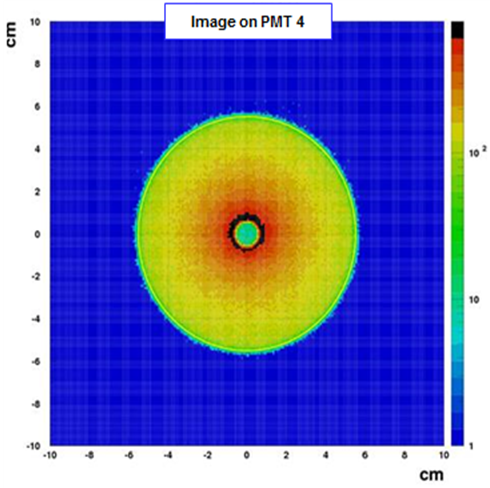
\includegraphics[width=1.0\linewidth,trim={0.0cm 0.0cm 0.0cm 0.0cm},clip]{images/Point_Targ_Zero_Field_PMT.png}
    \caption{Simulation result for the light collection pattern on the face of the PMT for a point-like target with no
      solenoidal field.}
    \label{fig:Point_Targ_Zero_Field_PMT}
\end{figure}

\begin{figure}[!ht]
    \centering
    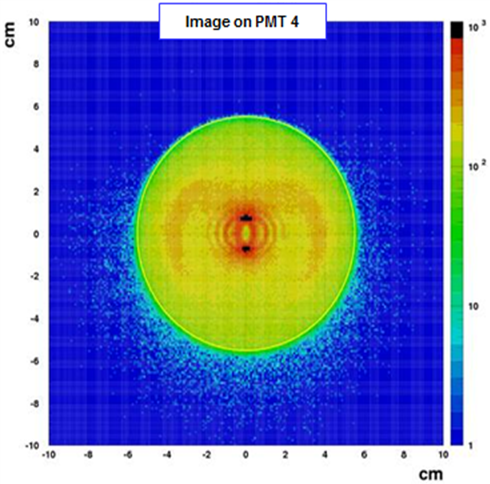
\includegraphics[width=1.0\linewidth,trim={0.0cm 0.0cm 0.0cm 0.0cm},clip]{images/Point_Targ_5T_Field_PMT.png}
    \caption{Simulation result for the light collection pattern on the face of the PMT for a point-like target and a 5~T
      solenoidal field.}
    \label{fig:Point_Targ_5T_Field_PMT}
\end{figure}

\begin{figure}[!ht]
    \centering
    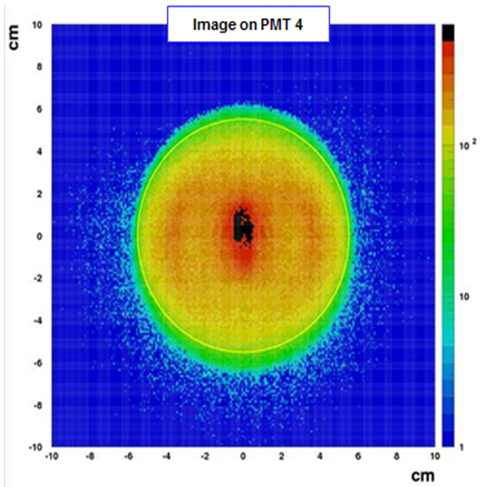
\includegraphics[width=1.0\linewidth,trim={0.0cm 0.0cm 0.0cm 0.0cm},clip]{images/10cm_Targ_5T_Field_PMT.png}
    \caption{Simulation result for the light collection pattern on the face of the PMT for a 10-cm-long target and 5~T
      solenoidal field.}
    \label{fig:10cm_Targ_5T_Field_PMT}
\end{figure}

\begin{figure}[!ht]
    \centering
    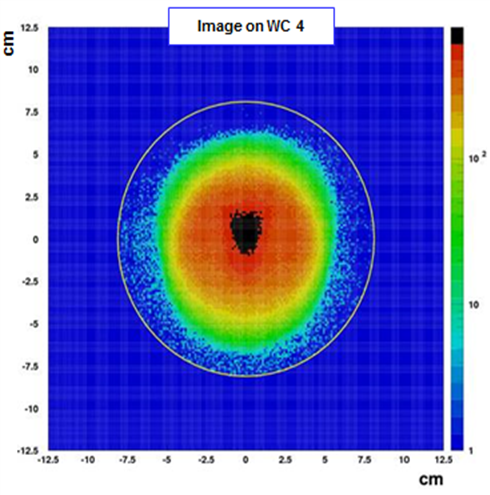
\includegraphics[width=1.0\linewidth,trim={0.0cm 0.0cm 0.0cm 0.0cm},clip]{images/10cm_Targ_5T_Field_WCone.png}
    \caption{Simulation result for the light collection pattern on the face of the Winston cone for a 10-cm-long target
      and a 5~T solenoidal field.}
    \label{fig:10cm_Targ_5T_Field_WCone}
\end{figure}

Estimates for the signal strength for 2~GeV electrons have been obtained for the point-like and extended targets
with and without the 5~T solenoid field. Figures~\ref{fig:Point_Targ_Zero_Field_Theta}, 
~\ref{fig:Point_Targ_5T_Field_Theta}, and ~\ref{fig:10cm_Targ_5T_Field_Theta} show angular distributions of
the signal strength. The corresponding plots of the signal strength in the azimuthal angle range are shown in
Figs.~\ref{fig:Point_Targ_Zero_Field_Phi}, ~\ref{fig:Point_Targ_5T_Field_Phi}, and 
~\ref{fig:10cm_Targ_5T_Field_Phi}. One can see that the signal strength increases with the polar angle. This
is because the electrons scattered at a smaller angle travel a shorter distance in the radiator gas as compared to
the electrons moving at larger angles. The minimum signal strength is estimated to be about 14-15 photoelectrons.
For electrons scattered in the range of polar angles from $5^\circ$ to $35^\circ$ we have a complete and uniform
coverage of the entire 2$\pi$ acceptance, as demonstrated by the azimuthal dependencies. The average signal
strength is about 17 photoelectrons. This estimate has been obtained by taking into account the possible reduction of
the mirror reflectivity due to the unavoidable influence of the hard to control factors during the detector construction
(dust and fume deposition, mechanical imperfections of the reflective surfaces, etc.) that were first observed during
the construction and maintenance of the CLAS Low Threshold Cherenkov Counter~\cite{Adams:2001kk}.

\begin{figure}[!ht]
    \centering
    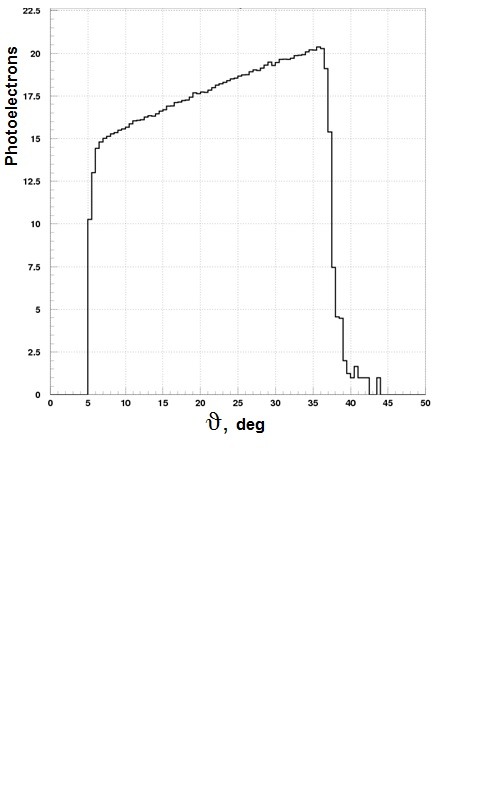
\includegraphics[width=1.0\linewidth,trim={0.0cm 9.4cm 0.0cm 0.0cm},clip]{images/Point_Targ_Zero_Field_Theta.jpg}
    \caption{Simulation results for the signal strength as a function of polar angle. Point-like target and no solenoidal
      field.}
    \label{fig:Point_Targ_Zero_Field_Theta}
\end{figure}

\begin{figure}[!ht]
    \centering
    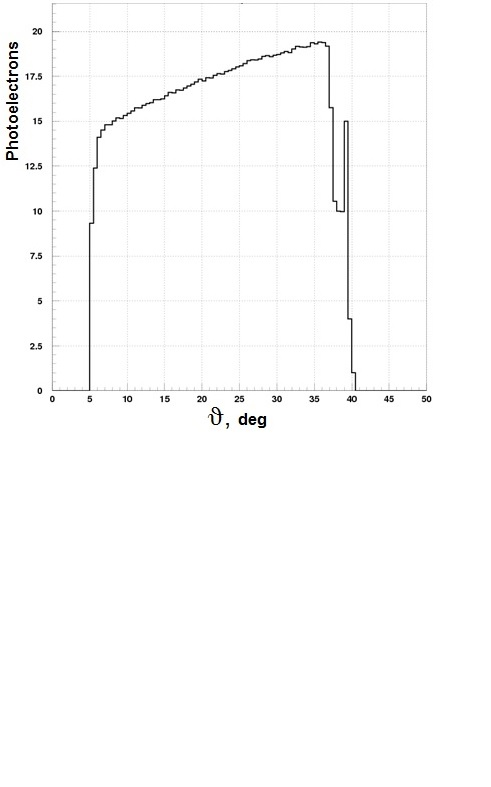
\includegraphics[width=1.0\linewidth,trim={0.0cm 9.4cm 0.0cm 0.0cm},clip]{images/Point_Targ_5T_Field_Theta.jpg}
    \caption{Simulation results for the signal strength as a function of polar angle. Point-like target with a 5~T
      solenoidal field.}
    \label{fig:Point_Targ_5T_Field_Theta}
\end{figure}

\begin{figure}[!ht]
    \centering
    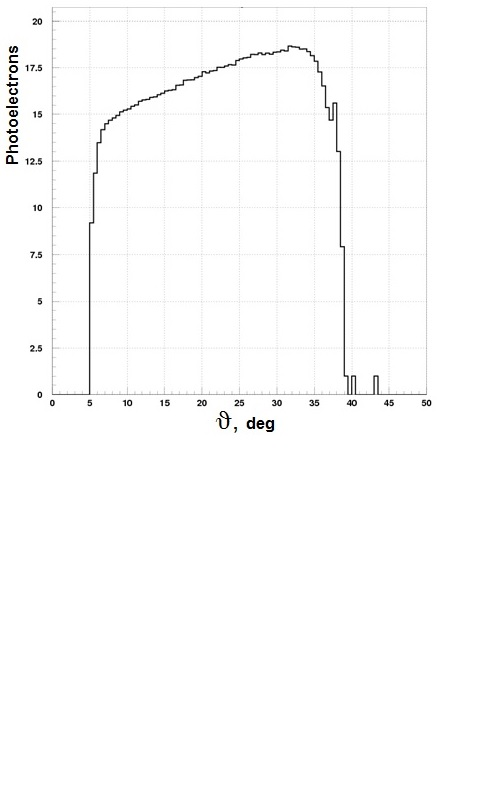
\includegraphics[width=1.0\linewidth,trim={0.0cm 9.4cm 0.0cm 0.0cm},clip]{images/10cm_Targ_5T_Field_Theta.jpg}
    \caption{Simulation results for the signal strength as a function of polar angle. 10-cm-long target with a 5~T
      solenoidal field.}
    \label{fig:10cm_Targ_5T_Field_Theta}
\end{figure}

\begin{figure}[!ht]
    \centering
    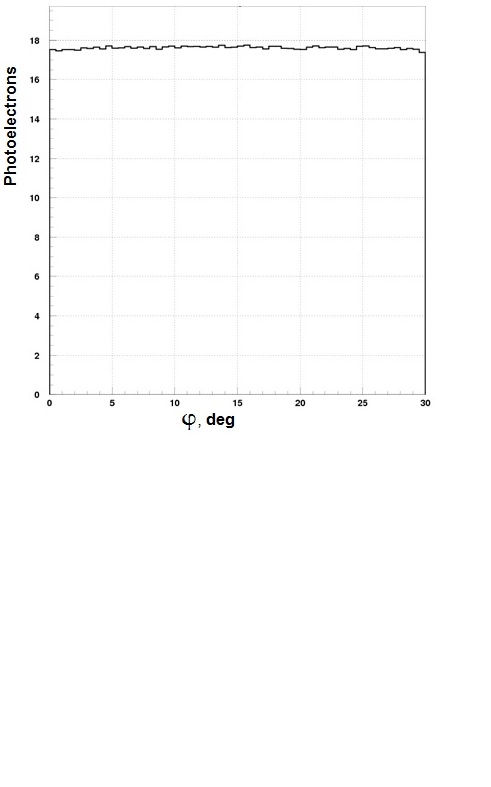
\includegraphics[width=1.0\linewidth,trim={0.0cm 9.4cm 0.0cm 0.0cm},clip]{images/Point_Targ_Zero_Field_Phi.jpg}
    \caption{Simulation results for the signal strength as a function of azimuthal angle. Point-like target with no
      solenoidal field.}
    \label{fig:Point_Targ_Zero_Field_Phi}
\end{figure}

\begin{figure}[!ht]
    \centering
    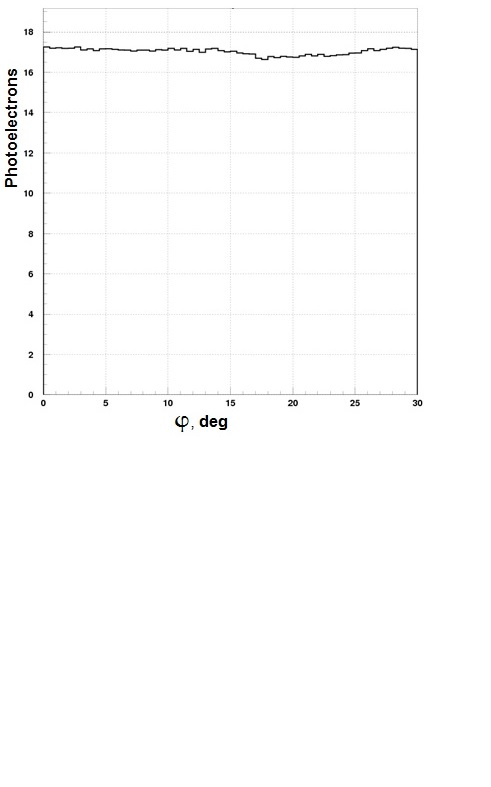
\includegraphics[width=1.0\linewidth,trim={0.0cm 9.4cm 0.0cm 0.0cm},clip]{images/Point_Targ_5T_Field_Phi.jpg}
    \caption{Simulation results for the signal strength as a function of azimuthal angle. Point-like target with 5~T
      solenoidal field.}
    \label{fig:Point_Targ_5T_Field_Phi}
\end{figure}

\begin{figure}[!ht]
    \centering
    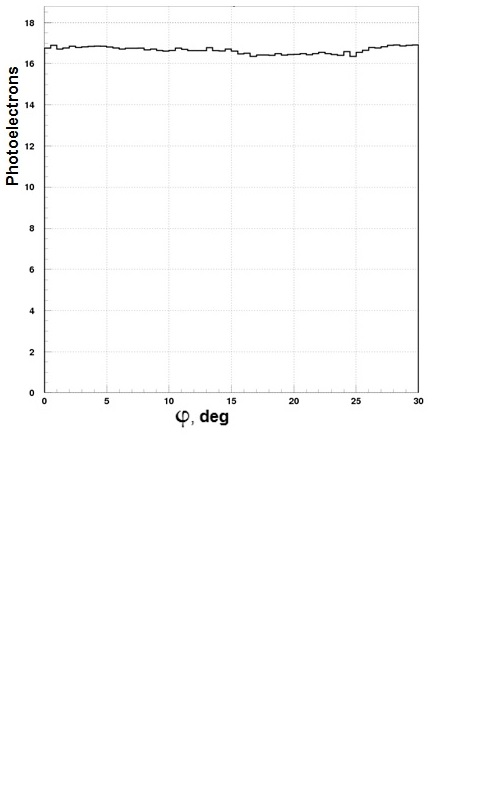
\includegraphics[width=1.0\linewidth,trim={0.0cm 9.4cm 0.0cm 0.0cm},clip]{images/10cm_Targ_5T_Field_Phi.jpg}
    \caption{Simulation results for the signal strength as a function of azimuthal angle. 10-cm-long target with 5~T
      solenoidal field.}
    \label{fig:10cm_Targ_5T_Field_Phi}
\end{figure}

One of sources of background events in the HTCC is the secondary interactions of charged pions with components
in the volume of the HTCC and with components outside the detector in the region between the target and the
HTCC entry window. Charged pions with energies mostly below the detection threshold can knock out relativistic
$\delta$ electrons that generate Cherenkov light in the HTCC volume. Some of that light can be focused by the
mirror on the PMTs. In our MC simulations we estimated the expected background rates. Of course the rates
depend on the actual thickness and distribution of the materials. We have specified in detail  everything regarding
the detector components in the simulation. With regard to outside components, we have taken into account the
10-cm-long cryogenic target filled with hydrogen, standard foam scattering chamber, and the air gap between the
exit window of the chamber and the entry window of the HTCC. At the CLAS12 design luminosity of
$\approx$ 10$^{35}$~cm$^{-2}$~s$^{-1}$, the estimated total background rate for one half-sector is about
20~kHz.

The most important parameters for the HTCC are the electron detection efficiency and the charged pion rejection
power. In Fig.~\ref{fig:Pion_rejection_2GeV} the simulation results on the rejection of charged pions are shown.
Data are presented for four HTCC channels from one half-sector at three different thresholds of electron
detection at 2~GeV: equivalent of 1, 2, and 3 photoelectrons. For the highest electron detection threshold ($\ge$3
photoelectrons) the estimated electron detection efficiency is 99.9\%. Similar results for 4~GeV electrons are
shown in Fig.~\ref{fig:Pion_rejection_4GeV}. One can conclude that at a threshold of 3 photoelectrons, the
average rejection factor is greater than 1000 at 2~GeV and at least 500 at 4~GeV, with an electron detection
efficiency close to 100\%.

\begin{figure}[!ht]
    \centering
    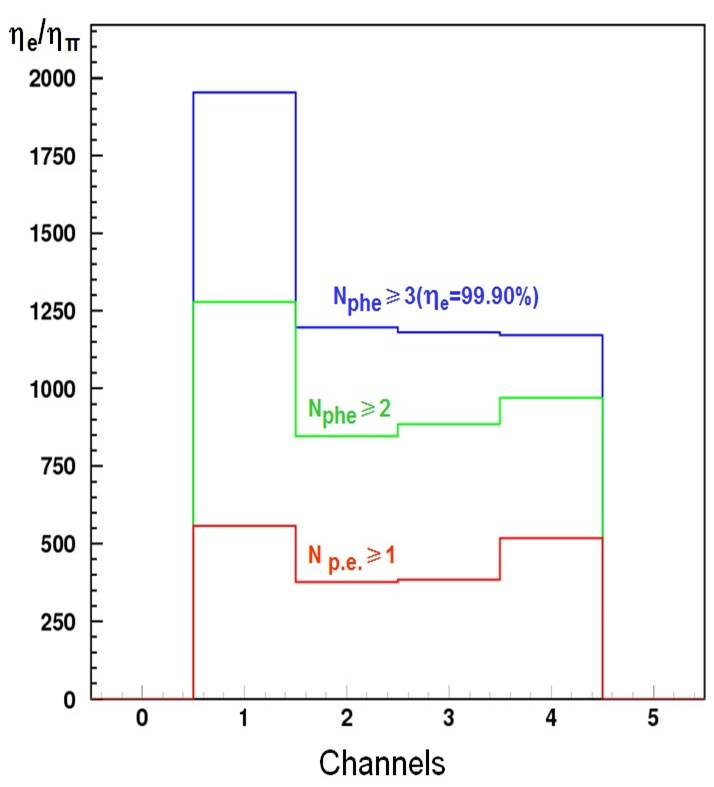
\includegraphics[width=1.0\linewidth,trim={0.0cm 0.0cm 0.0cm 0.0cm},clip]{images/Pion_rejection_2GeV.jpg}
    \caption{Rejection of charged pions at 2~GeV from Monte Carlo studies.}
    \label{fig:Pion_rejection_2GeV}
\end{figure}

\begin{figure}[!ht]
    \centering
    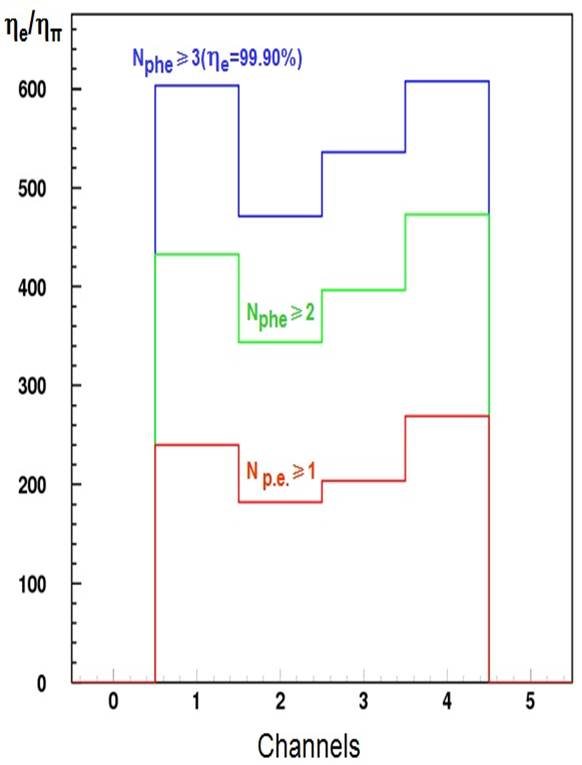
\includegraphics[width=1.0\linewidth,trim={0.0cm 0.0cm 0.0cm 0.0cm},clip]{images/Pion_rejection_4GeV.jpg}
    \caption{Rejection of charged pions at 4~GeV from Monte Carlo studies.}
    \label{fig:Pion_rejection_4GeV}
\end{figure}
